\seccion{Unas identidades y desigualdades}
\label{s:SZ:Desigualdades}

% Libro Loss Ruskai [Lieb]

\SZ{Desigualdades de Fano? Rioul p.  78, Cover P.~663, Sanov? Pythagorean? Gene:
  cf Zyc p60}

% ================================= MaxEnt

\subseccion{El principio de entrop\'ia m\'axima}
\label{sec:SZ:MaxEnt}

En la termodynamica, el estudio de las caracteristicas macroscopias (dynamica de
las  moleculas) es prohibitivo  tan el  numero de  moleculas es  importante. Por
ejemplo,  un  litro  del  gas  que  respiramos  contiene  $2.7  \times  10^{22}$
moleculas. De esta constataci\'on se desaroll\'o la f\'isica estad\'isticas bajo
el    impulso    de    Boltzmann~\cite{Bol96,   Bol98},    Maxwell~\cite{Max67},
Gibbs~\cite{Gib02},  Planck~\cite{Pla15}  entre  otros (see  also~\cite{Jay65}),
considerando el  sistema macroscopico  a trav\'es de  lo que  llamaron ensembles
esdadisticos:  el  sistema  global  (macroscopio)  es  al  equilibrio  pero  las
configuraciones (micro-estados)  son flucuantes. Se una forma,  se puede asociar
una  configuraci\'on  por su  frecuencia  de  ocurrencia  (imaginando tener  une
infinidad de  copias del sistema  en el mismo  estado macroscopio), es  decir su
probabilidad de occurencia.  En este marco, la entrop\'ia, describiendo la falta
de informaci\'on, juega un rol  fundamental.  Un sistema sujeto a vinculos, como
por  ejemplo teniendo  una  energia dada,  debe  estar en  sus  estado lo  m\'as
desorganizado dandos  los vinculos.   En su marco,  se introdujo la  noci\'on de
entrop\'ia  termodynamica,  pero  la  misma  es  tremendamente  vinculada  a  la
entrop\'ia   de   Shannon   (claramente,   identificando   las   frecuencias   a
probabilidades  de ocurrencia)~\footnote{Ver  ep\'igrafe  del cap\'itulo\ldots}.
En otro terminos,  la distribuci\'on describiendo los micro-estados  debe ser de
entrop\'ia m\'axima, dando los vinculos.  Por ejemplo, en un gas perfecto, donde
las particulas  no interactuan (aparte chocandose),  la energia es  dada por las
velocidades (suma  de las energias  cineticas individuales).  Dando  una energia
fija, la distribuci\'on de las  velocidad debe ser de entrop\'ia m\'axima sujeto
a  la  energia  dada  (nada  m\'as   que  la  energia  va  a  ``organizar''  las
configuraciones  posibles).   Intuitivamente,  en  un  sistema  aislado  de  $N$
particulas,  las  configuraciones  van  a  ser  equiprobables,  precisamente  la
distribuci\'on    maximizando   la   entrop\'ia.     \SZ{   En    la   secci\'on
  Sec.~\ref{sec:SZ:GasPerfecto} se va a desarollar un poco m\'as este ejemplo.}

De  manera general,  el problema  se formaliza  como la  buscada de  la entrop\'ia
m\'axima sujeto  a vinculos. Si  este principio naci\'o en  mecanica estad\'istica
(ver  tambi\'en~\cite{Jay57,  Jay57:2, Jay65}),  encontr\'o  un  echo en  varios
dominio:   en   inferencia   bayesiana   para  elegir   distribuciones   del   a
priori~\footnote{A partir  de una distribuci\'on parametrizada  por un parametro
  $\theta$.  El  enfoque de bayesiano  consiste a modelizar  $\theta$ aleatorio,
  digamos  $\Theta$,  tal que  la  distribuci\'on  de  observaciones se  escribe
  entonces  $p_{X|\Theta}$.   Inferir $\theta$  a  partir  de observaciones  $x$
  consiste   a   determinar  la   distribuci\'on   dicha   {\it  a   posteriori}
  $p_{\Theta|X}$.  Por  eso, hace  falta darse una  distribuci\'on dicha  {\it a
    priori} $p_\Theta$.   Si se conocen  momentos por una  razon o una  otra, se
  puede  elegir esta  distribuci\'on la  ``menos informativa''  posible,  \ie de
  entrop\'ia  m\'axima dados  los momentos.\label{foot:SZ:Prior}}  conociendo unos
momentos  de  la  ley~\cite{Rob07,  Jay68,  Jay82,  Csi91},  hacer  estimaci\'on
espectral  o de procesos  estocasticos autoregesivos~\cite{Bur67,  Bur75, Jay82}
o~\cite[cap.~12]{CovTho06}, entre otros~\cite[\& ref.]{KapKes92}.

Sea $X$ variable aleatoria viviendo  sobre $\X \subset \Rset^d$ con $K$ momentos
\  $\Esp\left[ M_k(X)  \right]  = m_k$  \ fijos,  con  $M_x: \X  \to \Rset$,  el
problema  de entrop\'ia  m\'axima se  formula de  la manera  siguiente en  el caso
continuo (es el caso discreto, hay que re-emplazar integrales por sumas): sean \
$M(x) = \begin{bmatrix} 1  & M_1(x) & \cdots & M_K(x) \end{bmatrix}^t$  \ y \ $m
= \begin{bmatrix} 1 & m_1 & \cdots & m_K \end{bmatrix}^t$, \ se busca,
%
\[
p^* = \argmax_p H(p) \qquad \mbox{sujeto a} \qquad p \ge 0, \quad \int_\X M(x)
\, p(x) \, dx = m
%1, \quad \int_X M_k(x) \, p(x) \, dx = m_k, \: k = 1, \ldots , K
\]
%
donde   los  dos  primeros   vinculos  aseguran   de  que   $p^*$  (positividad,
normalizaci\'on) sea una distribuci\'on de  probabilidad. En el ejemplo del gas,
$K =  1, M_1(x) = \sum_i  x_i^2$ (los $x_i$ son  las velocidades). Introduciendo
factores de Lagrange $\lambda = \begin{bmatrix} \lambda_0 & \lambda_1 & \cdots &
  \lambda_K  \end{bmatrix}^t$ para  tener en  cuenta los  vinculos,  el problema
variacional   consiste  a   resolver~\cite{GelFom63,  Bru04,   Mil00,  CamMar09,
  CovTho06}
%
\[
p^* = \argmax_p \int_\X \left( - p(x) \log p(x) + \lambda^t M(x) \, p(x) \right)
dx
\]
%
donde  $\lambda$  ser\'a  determinado  para  satisfacer  los  vinculos.   De  la
ecuaci\'on  de Euler-Lagrange~\cite{GelFom63, Bru04},  esquematicamente anulando
la ``derivada''  del integrande con respeto  a $p$ (sera  realmente un gradiente
los componentes  de $p$ en el  caso discreto), reparametrizando  los factores de
Lagrange, se obtiene
%
\[
p^*(x) = \e^{\lambda^t M(x)}
\]
%
con $\lambda$ tal que se  satisfacen los vinculos de normalizaci\'on y momentos.
Esta distribuci\'on  cae en la  familia conocida como {\it  familia exponencial}
donde  los  $M_k$  son  conocidos  como {\it  esdadisticas  suficientes}  y  los
$\lambda_k$  {\it   parametros  naturales}~\cite{Dar35,  Koo36,   And70,  Kay93,
  LehCas98, Rob07}.

Un problema que  puede aparecer es que no se puede  determinar $\lambda$ tal que
se  satisfacen todos  los vinculos,  en particular  la de  normalizaci\'on.  Por
ejemplo, si $\X = \Rset$ y $K = 0$, \ $p$ \ deberia ser constante (ley uniforme)
sobre\ldots $\Rset$, lo que no es normalizable. De la misma manera, si $K = 3$ \
y \ $M_k(x)  = x^k$, tampoco es normalizable  la funci\'on obtenida~\footnote{En
  el enfoque Bayesiano  se puede que no sea problematico, si  el a posteriori es
  normalizable~\cite{Rob07}, pero va m\'as all\'a  de la meta de esta secci\'on.}.
En otros terminos,  en este caso, el problema  no tiene soluci\'on~\footnote{M\'as
  precisamente,  existen casos en  los cuales  se puede  acotar la  entrop\'ia por
  arriba por un $H^{\sup}$, tal que  $\sup_p H(p) \le H^{\sup}$ pero no se puede
  alcanzar     esta     cota,     \ie      es     un     supremum,     no     un
  m\'aximo~\cite[sec.~12.3]{CovTho06}.}.

Existe una prueba informacional de este resultado, saliendo de la soluci\'on:
%
\begin{lema}
  Sea \ $\displaystyle \P_m = \left\{ p \ge 0: \: \int_\X M_k(x) \, p^*(x) \, dx
    =  m \right\}$ \  y \  $p^* \in  \P_m$ \  que sea  de la  forma \  $p^*(x) =
  \e^{\lambda^t M(x)}$. Entonces
  %
  \[
  \forall \,  p \in \P_m, \quad  H(p) \le H(p^*) \qquad  \mbox{con igualdad ssi}
  \quad p = p^*
  \]
  %
\end{lema}
\begin{proof}
\begin{eqnarray*}
H(p) & = & - \int_\X p(x) \, \log p(x) \, dx\\[2.5mm]
%
& = & - \int_\X p(x) \, \log\left( \frac{p(x)}{p^*(x)} \right) \, dx - int_\X
p(x) \, \log p^*(x) \, dx
\end{eqnarray*}
%
De $\log p^* = \lambda^t M$ se obtiene
%
\begin{eqnarray*}
H(p) & = & - D\left( p \left\| p^* \right. \right) - \int_\X \lambda^t M(x) p(x)
\, dx\\[2.5mm]
%
& = & - D\left( p \left\| p^* \right. \right) - \int_\X \lambda^t M(x) \, p^*(x)
\, dx\\[2.5mm]
%
& = & - D\left( p \left\| p^* \right. \right) - \int_\X p^*(x) \log p^*(x) \,
dx\\[2.5mm]
%
& = & - D\left( p \left\| p^* \right. \right) + H(p^*)
\end{eqnarray*}
%
porque $p,  p^* \in \P_m$ \  y \ $\lambda^t M  = \log p^*$. La  prueba se cierra
notando que $D \ge 0$ con igualdad si y solamente si $p = p^*$.
\end{proof}
%
Este lema prueba que, dando  vinculos ``razonables'', la entrop\'ia es acotada por
arriba,  y  que  se alcanza  la  cota  para  una  distribuci\'on de  la  familia
exponencial. Por ejemplo,
%
\begin{itemize}
\item Con  $K =  0$ \  y \  $\X$ \ de  volumen finito  \ $|\X|  < +  \infty$, la
  distribuci\'on  de entrop\'ia  m\'axima es  la distribuci\'on  uniforme  de la
  propiedad~\ref{prop:SZ:cotamaximauniforme}                            secci\'on
  Sec.~\ref{sec:SZ:Diferencial}      en       el      caso      continuo,      o
  propiedad~\ref{prop:SZ:cotamaxima}                                    secci\'on
  Sec.~\ref{sec:SZ:DefinicionShannon} en el caso discreto.
%
\item Con  $K =  1$, \ $\X  = \Rset^d$  \ y \  $M(x) = x  x^t$ (visto  con $d^2$
  vinculos),  la  distribuci\'on de  entrop\'ia  m\'axima  es la  distribuci\'on
  gausiana    de   la    propiedad~\ref{prop:SZ:cotamaximagaussiana}   secci\'on
  Sec.~\ref{sec:SZ:Diferencial}.
\end{itemize}


% ================================= EPI

\subseccion{Desigualdad de la potencia entr\'opica}

Sean $X$  e $Y$ dos variables indepedientes.  Si se sabe las  relaciones entre \
$H(X,Y)$, \ $H(X)$,  \ $H(Y)$, una pregunta natural  concierna la relaci\'on que
podrian tener $X+Y$ con cada variable en termino de entrop\'ia. La respuesta no es
trivial, y el  resultado general concierna el caso  de variables continuas sobre
$\Rset^d$.   Es conocido  como desigualdad  de la  potencia entr\'opica  (EPI para
entropy power  inequality en ingl\'es). No  vincula las entrop\'ias,  sino que las
potencias entr\'opicas.
%
\begin{teorema}[Desigualdad de la potencia entr\'opica]
  Sean  $X$  e  $Y$  dos variables  $d$-dimensionales  continuas  indepedientes,
  entonces
  %
  \[
  N(X + Y) \ge N(X) + N(Y)
  \]
%
  con  igualdad  sii  $X$  e  $Y$  son gaussianas  con  matrices  de  covarianza
  proporcionales,  $\Sigma_Y \propto  \Sigma_X$ (siempre  verdad en  el contexto
  escalar).
\end{teorema}
%
\noindent     Existen    varias     formulaciones     alternativas    a     esta
desiguladad~\cite{Sha48, Lie78, CovTho06, DemCov91, Rio07}:
%
\begin{enumerate}
\item\label{EPI:SZ:EquivGauss} Sean $\widetilde{X}$ y $\widetilde{Y}$ gaussianas
  independientes   de   matriz   de   covarianza  proporcionales   y   tal   que
  $H(\widetilde{X}) =  H(X)$ y $H(\widetilde{Y}) = H(Y)$.  Entonces
  %
  \[
  N(X+Y) \ge N\left( \widetilde{X} + \widetilde{Y} \right)
  \]
  %
  con igualdad sii $X$ y $Y$ son gaussianas.
%
\item\label{EPI:SZ:PresCov}    {\it    Desigualdad    de    preservaci\'on    de
    covarianza:}
  %
  \[
  \forall  \,   0  \le  \lambda  \le   1,  \quad  H\left(   \sqrt{\lambda}  X  +
    \sqrt{1-\lambda} Y \right) \ge \lambda H(X) + (1-\lambda) H(Y)
  \]
  %
  con igualdad el el caso gaussiano con matrices de covarianza proporcionales.
\end{enumerate}
%
%\noindent La  forma del teorema implica la  forma~\ref{EPI:SZ:PresCov} tomando \
%$\sqrt{\lambda} X$ \ y  \ $\sqrt{1-\lambda} Y$ \ en lugar de \ $X$  \ e \ $Y$, y
%recordandose que \ $N(a X) =  a^2 N(X)$. Reciprocamente, la forma del teorema se
%recupera de la forma~\ref{EPI:SZ:PresCov} tomando \ $\lambda = \frac12$.

La prueba  de esta(s) desigualdad(es) no es  trivial.  Numeras versiones
existen,  dadas por  ejemplo  en las  referencias~\cite{Bla65, Sta59,  ShaWea64,
  Rio07,  Rio11,  Rio17,  CovTho06,  DemCov91,  Lie78,  VerGuo06}  (ver  tambien
teorema~6  de~\cite{Lie75}) entre  otros.  Como  se lo  puede ver,  la gaussiana
juega un rol particular en esta desigualdad, saturandola.


\SZ{Ver si  es corto probar  la equivalencia entre  las tres formas.  Existe una
  forma, de Madiman, a traver rearreglo}

Esta desigualdad se usa para  probar otras desigualdades, como por ejemplo la
desigualdad de  Minkowsky $|R_1 +  R_2|^{\frac1d} \ge $ para  cualquieras matrices
$R_1,  R_2$ sim\'etricas  definidas positivas  (viene de  $X$ e  $Y$  gaussianas de
covarianza $R_1$  y $R_2$).  Aparece  tambi\'en para acotar  informaci\'on mutua
entre variables y  calcular la capacidad de un canal  de communicaci\'on como se
le va a ver~\cite{CovTho06, DemCov91, Rio07, Joh04}.

\SZ{En el caso discreto, no hay un resultado general.  Existent solamento
  resultados para variables particulares~\cite{toto, titi}.}


% ================================= Data Processing Theorem

\subseccion{Desigualdad de procesamiento de datos}

Esta  desigualdad  traduce  que  procesando  datos,  no  se  puede  aumentar  la
informaci\'on disponible sobre  una variable. Se basa sobre  una desigualdad que
satisface la informaci\'on mutua aplicada a un proceso de Markov.

\begin{definicion}[Proceso de Markov]
  Una secuencia  $X_1 \mapsto X_2 \mapsto  \ldots \mapsto X_n$ es  dicha {\it de
    Markov}   si   para  cualquier   $i   >   1$,
  %
  \[
  p_{X_{i-1},X_{i+1}|X_i} = p_{X_{i-1}|X_i} p_{x_{i+1}|X_i}
  \]
  %
  Dicho  de otra  manera, condicionalmente  a $X_i$,  las variables  $X_{i-1}$ y
  $X_{i+1}$       son       independientes.        Eso      es       equivalente
  a
  %
  \[
  p_{X_{i+1}|X_i,X_{i-1},\ldots} = p_{X_{i+1}|X_i}
  \]
  %
  Si  $i$  representa un  tiempo,  significa  que  la esdadistica  de  $X_{i+1}$
  conociendo todo el pasado se reduce  a esa conociendo el pasado inmediato (las
  probabilidades   dichas   de   transici\'on   $p_{X_{i+1}|X_i}$   caracterisan
  completamente  el proceso).   Es sencillo  fijar de  que $X_n  \mapsto X_{n-1}
  \mapsto \ldots \mapsto X_1$ es tambien un proceso de Markov.
\end{definicion}

\begin{teorema}[Desigualdad de procesamiento de datos]
  Sea  $X \mapsto  Y \mapsto  Z$ un  proceso de  Markov. Entonces,
  %
  \[
  I(X;Y) \ge I(X;Z)
  \]
  %
  con igualdad sii $X \mapsto Z \mapsto Y$ es tambi\'en un proceso de Markov. En
  particular, es  sencillo ver  que para cualquiera  funci\'on $g$, $X  \mapsto Y
  \mapsto g(Y)$ es un proceso de Markov,  lo que da
  %
  \[
  \forall \, g, \quad I(X;Y) \ge I(X;g(Y))
  \]
  %
  La  \'ultima  desigualdad  se  escribe  tambi\'en  $H(X|g(Y))  \ge  H(X|Y)$  y
  significa que  procesar $Y$ no aumenta  la informaci\'on que $Y$  da sobre $X$
  (la incerteza condicional es m\'as importante).
\end{teorema}
%
\begin{proof}
  Por definici\'on  de la  informaci\'on mutua, considerando  $X$ y  la variable
  conjunta $(Y,Z)$,
%
\begin{eqnarray*}
I(X ; Y,Z) & = & H(X) - H(X|Y,Z)\\[2.5mm]
%
& = & H(X) - H(X|Y) + H(X|Y) - H(X|Y,Z)
\end{eqnarray*}
%
\noindent Por la propiedad que $Z  \mapsto Y \mapsto X$ sea tambi\'en un proceso
de Markov, es sencillo probar que $H(X|Y,Z) = H(X|Y)$ (conciendo $Y$ sufice para
caracterisar completamente $X$), lo que da
%
\[
I(X;Y,Z) = I(X;Y)
\]
%
Tambi\'en,
%
\begin{eqnarray*}
I(X ; Y,Z) & = & H(X) - H(X|Z) + H(X|Z) - H(X|Y,Z)\\[2.5mm]
%
& = & I(X;Y) + H(X|Z) - H(X|Y,Z)
\end{eqnarray*}
%
\noindent  Adem\'as,   escribiendo  $\frac{p_{X|Y,Z}}{p_{X|Z}}  =  \frac{p_{X|Y,Z}
  p_{Y|Z}}{p_{X|Z} p_{Y|Z}} = \frac{p_{X,Y|Z}}{p_{X|Z} p_{Y|Z}}$
% $H(X|Z) -  H(X|Y,Z) \Esp\left[ \log \left(
% \frac{p_{X|Y,Z}(X,Y,Z)}{p_{X|Z}(X,Z)}\right)\right] = $
%& = & \int p_{X,Y,Z} \log \left(
%  \frac{p_{X|Y,Z}}{p_{X|Z}} \right)\\[2.5mm]
%%
%& = & \int p_{X,Y,Z} \log \left( \frac{p_{X|Y,Z}
%    p_{Y|Z}}{p_{X|Z}   p_{Y|Z}}   \right)\\[2.5mm]
%%
%& = &   \int   p_{X,Y,Z}   \log   \left(
%  \frac{p_{X,Y|Z}}{p_{X|Z}  p_{Y|Z}}  \right)
%\end{eqnarray*}
%
%\noindent  (y  similaramente  en  el   caso  discreto)  
%Calculos sencillos,
se muestra  que $H(X|Z)  - H(X|Y,Z)$ es  una divergencia de  Kullback-Leibler de
$p_{X,Y|Z}$ relativamente a $p_{X|Z}  p_{Y|Z}$, o informaci\'on mutua $I(X;Y|Z)$
entre \ $X$ \ e \ $Y$,  condicionalmente a \ $Z$).  Entonces
%
\[
I(X;Y) = I(X;Z) + I(X;Y|Z)
\]
%
lo  que  proba  la  desigualdad  del   hecho  de  que  una  divergencia  sea  no
negativa. Adem\'as, se obtiene la igualdad sii  $I(X;Y|Z) = 0$, es decir $X$ e $Y$
independientes  condicionalmente a  $Z$, lo  que es  la definici\'on  de  que $X
\mapsto Z \mapsto Y$ sea un proceso de Markov.
\end{proof}

% ================================= Data Processing Theorem

\subseccion{Secunda ley de la termodinamica}

Tratando de procesos  de Markov, aparece el equivalente de la  secunda ley de la
termodinamica:  un  sistema  aislado  evolua  hasta  llegar  su  estado  lo  m\'as
desorganizado.

\begin{lema}[ver~\cite{CovTho06}]
  Sea $X_1 \mapsto X_2 \mapsto \cdots  \mapsto X_n \mapsto \cdots$ un proceso de
  Markov,  con probabilidades  de transici\'on  $p_{X_{n+1}|X_n}$  dadas.  Estas
  modelan  el sistema,  independiente de  las condiciones  iniciales.   Sean dos
  distribuciones (condiciones) iniciales diferentes $p_1$ y $q_1$, conduciendo a
  las distribuciones $p_n$ y $q_n$ para $X_n$. Entonces:
%
\begin{itemize}
\item  Para cualquier  $n \ge  1$,
  %
  \[
  D(p_{n+1}\|q_{n+1}) \le D(q_n\|p_n)
  \]
  %
  las distribuciones $p_n$ y $q_n$ no se ``alejan'' (tiende a acercarse);
%
\item  Si  $p^*$  es  una  distribuci\'on  estacionaria,
  %
  \[
  D(p_{n+1}\|p^*) \le D(p_n\|p^*)
  \]
  %
  la distribuci\'on no se aleja de la distribuci\'on estacionaria.
%
\item Adem\'as, si  los $X_n$ viven sobre  $\X$ de cardinal o volumen  finito y si
  $p^*$ es  uniforme sobre $\X$,
  %
  \[
  H(X_{n+1}) \ge H(X_n)
  \]
  %
  el  sistema tiende  a desorganizarse  (y recuerdese  de que  la distribuci\'on
  uniforme es la de entrop\'ia m\'axima).
\end{itemize}
\end{lema}
%
\begin{proof}
  Escribiendo   $p_{n+1,n}$  y  $q_{n+1,n}$   las  distribuciones   conjunta  de
  $(X_{n+1},X_n)$  para   las  dos   condiciones  iniciales,  ,   $p_{n+1|n}$  y
  $q_{n+1|n}$  las  distribuciones  condicionales  de $X_{n+1}|X_n$  as\'i  que,
  $p_{n|n+1}$ y  $q_{n|n+1}$ las distribuciones  condicionales de $X_n|X_{n+1}$,
  se muestra sencillamente  que $D(p_{n+1,n}\|q_{n+1,n}) = D(p_{n+1}\|q_{n+1}) +
  D(p_{n+1|n}\|q_{n+1|n})  =  D(p_n\|q_n)  +  D(p_{n|n+1}\|q_{n|n+1})$.  Adem\'as,
  $p_{n+1|n}     =    p_{X_{n+1}|X_n}     =     q_{n+1|n}$,    conduciendo     a
  $D(p_{n+1|n}\|q_{n+1|n}) = 0$ y  entonces $D(p_{n+1}\|q_{n+1}) = D(p_n\|q_n) +
  D(p_{n|n+1}\|q_{n|n+1})$.   $p_{n|n+1}$   no   es   necesariamente   igual   a
  $q_{n|n+1}$,  pero la divergencia  siendo nonnegativa,  se obtiene  la primera
  desigualdad.  La secunda desigualdad se  obtiene tomando $q_n = p^*$.  Adem\'as,
  si $p^*$  es uniforme  $p^*(x) = \frac{1}{|\X|}$  da $D(p_n\|p^*) =  -H(X_n) +
  \log |\X|$, dando la \'ultima desigualdad.
\end{proof}


% ================================= Principop de incerteza

\subseccion{\SZ{Principio de incerteza entr\'opico}}

\SZ{Bourret 58, Leipnik 59 entre otros que ya citamos un par de veces}

% ================================= Fisher

\subseccion{Un foco sobre la informaci\'on de Fisher}

Si  la entrop\'ia  y las  heramientas relacionadas  son naturales  como  medida de
informaci\'on, no se  puede resumir una distribuci\'on a  una medida escalar. En
el marco  de la teor\'ia de la  estimaci\'on, R. Fisher introdujo  una noci\'on de
informaci\'on intimamente relacionada al  error cuadratico en la estimaci\'on de
un   parametro    a   partir   de   una   variable    parametrizado   por   este
parametro~\cite{Fis22,  Fis25:07,   Kay93,  Bos07,  CovTho06, Fri04}.

{\it Mencionamos que en esta secci\'on, se usar\'a el logaritmo natural.}
% , a pesar de que sea  necesarion solamente para la desigualdad de Cram\'er-Rao
% que se va a ver en unos parafos.}
%
\begin{definicion}[Matriz informaci\'on de Fisher parametrica]
  Sea $X$ una variable aleatoria parametrizada por un parametro $m$-dimensional,
  $\theta  \in  \Theta \subseteq  \Rset^m$,  de  distribuci\'on de  probabilidad
  $p_X(\cdot;\theta)$ continua  sobre $\X  \subseteq \Rset^d$ su  soporte. Asume
  que $p_X$ sea diferenciable en  $\theta$ sobre $\Theta$.  La matriz de Fisher,
  de tama\~no $m \times m$ es definida por
  %
  \[
  J_\theta(X)  =  \Esp\left[  \Big(  \nabla_\theta \log  p_X(X;\theta)  \Big)
    \Big( \nabla_\theta \log p_X(X;\theta) \Big)^t \right]
  \]
  %
  donde $\nabla_\theta = \left[  \cdots \: \frac{\partial}{\partial \theta_i} \:
    \cdots \right]^t$ es  el gradiente en $\theta$.  Es  la matriz de covarianza
  del  {\it score  parametrico} $S(X)  = \nabla_\theta  \log  p_X(X;\theta)$ (se
  proba que su promedio es  cero), siendo $\log p_X$ la {\it log-verosimilitud}.
  Bajo   condiciones   de  regularidad,   se   puede  mostrar~\footnote{Es   una
    consecuencia del  teorema de la  divergencia, suponiendo que los  bordes del
    dominio de $X$ no depende de $\theta$ y que la funci\'on score se cancela en
    estos  bordes.}  que  $J_\theta(X)$ es  tambi\'en  menos el  promedio de  la
  Hessiana~\footnote{Para $f:  \Rset^m \mapsto \Rset, \quad  \Hess_\theta f$ es
    la  matriz de  componentes $\frac{\partial^2  f}{\partial  \theta_i \partial
      \theta_j}$.}  $\Hess_\theta$ de  $\log  p_X(X;\theta)$.  Nota:  a veces  se
  define  la  informaci\'on  de  Fisher   como  $\Tr(J)$,  traza  de  la  matriz
  informaci\'on de Fisher.
\end{definicion}
%
Como  para   la  entrop\'ia,   la  matriz  de   Fisher  se   escribe  generalmente
$J_\theta(X)$, a  pesar de que no  sea funci\'on de  $X$ pero de la  densidad de
probabilidad. Se  la notara tambi\'en  $J_\theta(p_X)$ seg\'un la  escritura la
m\'as conveniente.

Tomando el gradiente  en $x$ en lugar de $\theta$ da  la matriz de informaci\'on
de Fisher no parametrica,
%
\begin{definicion}[Matriz informaci\'on de Fisher no parametrica]
  Sea  $X$  una  variable  aleatoria  de distribuci\'on  de  probabilidad  $p_X$
  definida  sobre  $\X \subseteq  \Rset^d$  su  soporte.   Asuma que  $p_X$  sea
  diferenciable (en $x$).   La matriz de Fisher no parametrica,  $d \times d$ es
  definida por
  %
  \[
  J(X) =  \Esp\left[ \Big(  \nabla_x \log p_X(X)  \Big) \Big(  \nabla_x \log
      p_X(X) \Big)^t \right]
  \]
  %
  Es la matriz de covarianza de  la {\it funci\'on score} $\nabla_x \log p_X(X)$
  (se  proba  que  su  promedio  tambi\'en  es  cero)  o,  bajo  condiciones  de
  regularidad, menos el promedio de la Hessiana en $x$ de la log-verosimilitud.
\end{definicion}
%
Es interesante notar que:
%
\begin{itemize}
\item Cuando $\theta$ es un  parametro de posici\'on, $p_X(x;\theta) = p(x -
\theta)$,  $\nabla_\theta \log p_X  = -  \nabla_x \log  p_X$ y  la informaci\'on
parametrica se reduce a la informaci\'on no parametrica.
%
\item  Si $X$  es  gaussiano de  matriz  de covarianza  $\Sigma_X$, entonces  se
  muestra sencillamente de que $J(X)  = \Sigma_X^{-1}$ (o, de una forma, inversa
  de la dispersi\'on o incerteza en termino de estad\'isticas de orden 2).
%
\item Es sencillo ver  que, por definici\'on \ $J_\theta(X)$ \ y  \ $J(X)$ \ son
  sim\'etricas  y  que \  $J_\theta(X)  > 0$  \  y  \ $J(X)  >  0$  \ donde  estas
  desiguladades  significan  que  las  matrices  son  definidas  positivas  (los
  autovalores son positivos).  Adem\'as,
  %
  \[
  \forall \ a \ne 0, \quad J(aX) = \frac{1}{|a|^2} J(X)
  \]
  %
  (queda v\'alido  para $a$  matriz invertible).  Esta  relaci\'on da a  $J(X)$ un
  sabor de  informaci\'on en el sentido  de que, cuando $a$  tiende al infinito,
  $J(aX)$  tiende a  0;  $a X$  tiende  a ser  muy diepersas  as\'i  que no  hay
  informaci\'on sobre su posici\'on.
%
\item $J_\theta$ \ y \ $J$ \ son  convexas en el sentido de que \ para cualquier
  conjunto de  $\lambda_k \ge  0, \sum_{k=1}^K  \lambda_k = 1$  \ y  \ cualquier
  conjunto    de   distribuciones    \   $p_k,    \    k   =    1,   \ldots    ,
  K$~\cite{Coh68, Fri04},
  %
  \[
  J_\theta\left(  \sum_{k=1}^K  \lambda_k  p_k  \right)  \:  <  \:  \sum_{k=1}^K
  \lambda_k  \,  J_\theta\left(  p_k  \right)  \qquad  \mbox{y}  \qquad  J\left(
    \sum_{k=1}^K \lambda_k  p_k \right) \:  < \: \sum_{k=1}^K  \lambda_k J\left(
    p_k \right)
  \]
%
  donde $A < B$ significa que $B-A$ es definida positiva.  La prueba es dada por
  Cohen en  el caso  escalar, pero se  extiende sin  costo adicional en  el caso
  multivariado. Hace falta  probarlo para $K=2$ y, por  recurrencia, se extiende
  por cualquier  $K$. En este  caso, observando que  $\big( \nabla \log  p \big)
  \big( \nabla \log p  \big)^t \, p = \frac{\big( \nabla p  \big) \big( \nabla p
    \big)^t}{p}$, considerando  el gradiente con respeto a  $\theta$ (resp. $x$)
  tratando de  $J_\theta$ (resp. $J$), se obtiene  $\sum_k \lambda_k \frac{\big(
    \nabla p_k \big) \big( \nabla p_k \big)^t}{p_k} - \frac{\left( \nabla \sum_k
      \lambda_k p_k \right) \left( \nabla \sum_k \lambda_k p_k \right)^t}{\sum_k
    \lambda_k  p_k} =  \frac{1}{\sum_k  \lambda_k p_k}  \, \sum_{k,l}  \lambda_k
  \lambda_l  \Big(  \frac{p_l}{p_k} \big(  \nabla  p_k  \big)  \big( \nabla  p_k
  \big)^t - \big( \nabla p_k \big)  \big( \nabla p_l \big)^t \Big)$, lo que vale
  (tratamos del caso  $K = 2$), $ \frac{\lambda_1  \lambda_2}{p_2 p_2 (\lambda_1
    p_1 + \lambda_2 p_2)} \big( p_2 \nabla  p_1 - p_1 \nabla p_2 \big) \big( p_2
  \nabla p_1  - p_1 \nabla p_2 \big)^t  \ge 0$. No puede  ser identicamente cero
  (salvo si $\lambda_1 \lambda_2 = 0$  o $p_1 = p_2$\ldots) as\'i que se obtiene
  la desigualdad sobre la matriz de Fisher integrando esta desigualdad.
\end{itemize}


Una otra interpretaci\'on  de $J$ como informaci\'on es  debido a la desigualdad
de  Cram\'er-Rao que  la vincula  a la  covarianza  de estimaci\'on~\footnote{De
  hecho,  pareci\'o esta  formula tambi\'en  en los  papeles de  Fr\'echet  y de
  Darmois~\cite{Fre43, Dar45}. Como citado por Fr\'echet, aparece que la primera
  versi\'on  de esta  formula  es mucho  m\'as vieja  y  debido a  K.  Pearson  \&
  Filon~\cite{PeaFil98} en 1898; luego fue extendido por Edgeworth~\cite{Edg08},
  Fisher~\cite{Fis25:07}  o  Doob~\cite{Doo36}.}~\cite{Rao45,  Rao92,  RaoWis47,
  Cra46,  Rio07, CovTho06,  Fri04,  Kay93, Bos07}.   Sea  $X$ parametrizada  por
$\theta$.  La meta es estimar $\theta$ a  partir de $X$.  Tal estimador va a ser
una  funci\'on unicamente  de $X$,  lo que  se  escribe usualmente~\footnote{Por
  ejemplo,  si $\theta$  es un  promedio com\'un  a los  componentes de  $X$, un
  estimador   podr\'ia   ser   $\widehat{\theta}   =   \frac1d   \sum_i   X_i$.}
$\widehat{\theta}(X)$ (la funci\'on no depende explicitamente de $\theta$).  Las
caractericas de la calidad de un  estimator es naturalmente su bias $b(\theta) =
\Esp\left[  \widehat{\theta}(X)  \right]  -   \theta$  y  su  matriz  covarianza
$\Sigma_{\widehat{\theta}}$  (la varianza  da  la dispersi\'on  alrededor de  su
promedio). La desigualdad de Cram\'er-Rao acota por debajo esta covarianza.
%
\begin{teorema}[Desigualdad de Cram\'er-Rao]
  Sea  $X$ parametrizada  por $\theta$,  de  densidad de  soporte $\X  \subseteq
  \Rset^d$  indendiente  de $\theta$  y  $\widehat{\theta}(X)$  un estimador  de
  $\theta$.  Sea $b(\theta)$ su  bias y $\Sigma_{\widehat{\theta}}$ su matriz de
  covarianza.   Sea   $\Jac_b(\theta)$  la   matriz  Jacobiana  del   bias  $b$.
  Entonces,
  %
  \[
  \Sigma_{\widehat{\theta}} - \left( I + \Jac_b(\theta) \right) J_\theta(X)^{-1}
  \left( I + \Jac_b(\theta) \right)^t \ge 0
  \]
  %
  En particular, en el  caso $\theta$ escalar,
  %
  \[
  \sigma_{\widehat{\theta}}^2 \ge \frac{(1+b'(\theta))^2}{J_\theta(X)}
  \]
  %
  donde  $b'$ es  la  derivada  de $b$.\newline  Tomando  $\theta$ parametro  de
  posici\'on y $\widehat{\theta}  = X$, estimador sin bias ($b =  0$), eso da lo
  que es conocido  como la desigualdad no parametrica de  Cram\'er-Rao y toma la
  expresi\'on
  %
  \[
  \Sigma_X - J(X)^{-1} \ge 0
  \]
  %
  o, en el caso escalar,
  %
  \[
  \sigma_X^2 \ge \frac{1}{J(X)}
  \]
  %
  Adem\'as, en el caso no parametrico, se alcanza la cota si y solamente si $X$ es
  un vector gaussiano.
\end{teorema}
%
\noindent Esta  desigualdad acota la variaza  de cualquier estimador,  \ie da la
varianza o error  m\'inima que se puede  esperar. Esta cota es el  inverso de la
informaci\'on de Fisher, \ie  $J_\theta(X)$ caracteriza la informaci\'on que $X$
tiene sobre $\theta$.
%
\begin{proof}
  Sea $S = \nabla_\theta \log  p_X$ y $\theta_0 = \Esp\left[ \widehat{\theta}(X)
  \right] = \theta + b(\theta)$. Fijandose  que $\nabla_\theta \log p_X \, p_X =
  \nabla_\theta p_X$, que $\widehat{\theta}$ no  es funci\'on de $\theta$, y que
  el soporte $\X$ no depende de $\theta$, se obtiene~\footnote{Se supone que los
    integrandes sean $\theta$-localmente integrables,  tal que se puede invertir
    derivada en $\theta$ e integraci\'on.}
  %
  \begin{eqnarray*}
  \Esp\left[ S(X) \left( \widehat{\theta}(X) - \theta_0 \right)^t \right] & = &
  \int_\X \nabla_\theta p_X(x;\theta) \widehat{\theta}(x)^t \, dx - \left(
  \int_\X \nabla_\theta p_X(x;\theta) \, dx \right) \theta_0^t\\[2.5mm]
  %
  & = & \nabla_\theta \int_{\Rset^d} p_X(x;\theta) \widehat{\theta}(x)^t \, dx -
  \left( \nabla_\theta \int_{\Rset^d} p_X(x;\theta) \, dx \right)
  \theta_0^t\\[2.5mm]
  %
  & = & \nabla_\theta \left( \theta + b(\theta) \right)  - 
  \left( \nabla_\theta 1 \right) \theta_0^t\\[2.5mm]
  %
  & = & \left( I + \Jac_b(\theta) \right)^t
  \end{eqnarray*}
  %
  Adem\'as,  fijandose  que  $\Esp\left[  S(X)  S(X)^t \right]  =  J_\theta(X)$  y
  $\Esp\left[   \left(    \widehat{\theta}(X)   -   \theta_0    \right)   \left(
      \widehat{\theta}(X)      -      \theta_0      \right)^t     \right]      =
  \Sigma_{\widehat{\theta}}$,            la            desigualdad            de
  Cauchy-Bunyakovsky-Schwarz~\footnote{De  hecho, fue  probada  por Cauchy  para
    sumas en 1821, para integrales por  Bunyakovsky en 1859 y m\'as elegamente por
    Schwarz  en  1888~\cite{Ste04}.}   conduce  a
  %
  \[
  \left( u^t \left( I + \Jac_b(\theta)  \right)^t v \right)^2 \: = \: \Esp\left[
    u^t S(X) \left( \widehat{\theta}(X) -  \theta_0 \right)^t v \right]^2 \: \le
  \: u^t J_\theta(X) u \: v^t \Sigma_{\widehat{\theta}} \, v
  \]
  %
  La prueba se termina tomando \ $u = J_\theta(X)^{-1} \left( I + \Jac_b(\theta)
  \right)^t \, v$ (recordandose que $J$ es sim\'etrica).\newline Con la elecci\'on
  de  $u$,  en  la  desigualdad  de Cauchy-Bunyakovsky-Schwarz,  se  obtiene  la
  igualdad  cuando, \  $v^t J(X)^{-1}  S(x)  \propto v^t  (x -  \theta)$ \  para
  cualquier \  $v$ \ y \  $x$, est decir \  $\nabla_x p_X (x) \propto  J(X) (x -
  \theta) p_X(x)$, lo que es la ecuaci\'on diferencial que satisface (solamente)
  la  gaussiana:   en  este  caso,  se   verifica  a  posteriori   que  $J(X)  =
  \Sigma_X^{-1}$,  y entonces  que  se alcanza  la  cota de  la Cram\'er-Rao  no
  parametrica.
\end{proof}
%
\noindent En el  caso parametrico, no se puede estudiar el  caso de igualdad del
hecho  de  que  $\widehat{\theta}$ no  es  algo  dado.   Adem\'as, a\'un  dado  un
estimador  (independiente explicitamente de  $\theta$), no  hay garantia  de que
existe  una  densidad parametrizado  por  $\theta$ que  alcanza  la  cota, o  al
rev\'es, dado una  familia de densidades, tampoco no hay  garantia que existe un
estimador que permite alcanzar la cota~\cite{CovTho06,  Kay93}.

Fijense de que, de nuevo, la gaussiana juega un rol particular en la desigualdad
de Cram\'er-Rao no parametrica , permitiendo alcanzar la cota.

Nota: para dos  matrices $A \ge 0$  \ y \ $B \ge  0$, si $A - B  \ge 0$ entonces
$|A|  \ge  |B|$,   con  igualdad  si  y  solamente   si  $A  =  B$~\cite[cap.~1,
teorema~25]{MagNeu99}.   Entonces,  de  las  desigualdades  de  Carm\'er-Rao  se
deducen     desigualdades     de     Cram\'er-Rao    escalares
%
\[
\left|   \Sigma_{\widehat{\theta}}  \right|   \,   \ge  \,   \frac{\left|  I   +
    \Jac_b(\theta) \right|^2}{\left| J_\theta(X) \right|} \qquad \mbox{y} \qquad
\left| \Sigma_X \right| \, \ge \, \frac{1}{\left| J(X) \right|}
\]
%
Obviamente,  en la secunda,  se alcanza  la igualdad  si y  solamente si  $X$ es
gaussiano.  Adem\'as,  para   una  matriz  $A  \ge  0$,   existe  la  ``relaci\'on
determinente-traza''  \ $|A|^{\frac1d} \le  \frac1d \Tr(A)$,  con igualdad  si y
solamente  si $A  = I$~\cite[cap.~11,  sec.~4]{MagNeu99}, dando  otras versiones
escalares de la desigualdad de Cram\'er-Rao, por ejemplo
% \Tr\left(\Sigma_{\widehat{\theta}}  \right)  \,  \ge  \, \frac{d^2  \,  \left(
%     \Tr\left(I   +  \Jac_b(\theta)  \right)   \right)^2}{\Trleft|  J_\theta(X)
% \right|} \qquad \mbox{y} \qquad
%
\[
\left| \Sigma_X  \right|^{\frac1d} \,  \ge \, \frac{d}{\Tr\left(  J(X) \right)},
\qquad   \Tr\left(   \Sigma_X   \right)   \,   \ge   \,   \frac{d}{\left|   J(X)
  \right|^{\frac1d}} \qquad \mbox{o} \qquad \Tr\left( \Sigma_X \right) \, \ge \,
\frac{d^2}{\Tr\left( J(X) \right)}
\]
%
En  estos casos,  se obtiene  la igualdad  si y  solamente si  $X$  es gaussiana
(igualdad de la Cram\'er-Rao no parametrica) y adem\'as de covarianza proporcional
a la identidad (igualdad en la relaci\'on determinente-traza).

Se notar\'a que,  al imagen de las leyes de  entrop\'ia m\'axima, la informaci\'on
de  Fisher  juega tambi\'en  un  rol particular  en  la  inferencia bayesiana  a
trav\'es del prior de Jeffrey~\cite{Jef46, Jef48, LehCas98, Rob07}~\footnote{Ver
  nota  de pie~\ref{foot:SZ:Prior}.   A  veces, se  toma  como distribuci\'on  a
  priori $p_\Theta(\theta) \propto  |J_\theta(X)|^\frac12$ por su invarianza por
  reparametrizaci\'on $\eta =  \eta(\theta)$, \ie el prior de  Jeffrey en $\eta$
  es uniquevocamente obtenido con la Fisher  en $\eta$ o por cambio de variables
  saliendo de $p_\Theta$.}.

\

Si  la  desigualdad de  Cram\'er-Rao  da  a la  matriz  de  Fisher  un sabor  de
informaci\'on,  aparece   que  $J$  es  tambi\'en  relacionado   a  la  entrop\'ia
relativa~\cite{CovTho06, Fri04}:
%
\begin{teorema}[Fisher como curvatura de la entrop\'ia relativa]
  Sea $X$  parametrizado por $\theta_0  \in \Theta$ con $\Theta$  conteniendo un
  vecinaje de $\theta_0$.  Siendo $\Dkl[p_X(\cdot;\theta)]{p_X(\cdot;\theta_0)}$
  funci\'on de $\theta \in \Theta$, aparece que
  %
  \[
  \Dkl[p_X(\cdot;\theta)]{p_X(\cdot;\theta_0)}   =  \frac12   \left(   \theta  -
      \theta_0  \right)^t J_{\theta_0}(X)  \left(  \theta -  \theta_0 \right)  +
    o\left( \| \theta - \theta_0 \|\right)
  \]
  %
  donde $o(\cdot)$ es un resto peque\~no  con respecto a su argumento.  En otros
  terminos,  $J_{\theta_0}(X)$  es  la  curvatura  de la  entrop\'ia  relativa  en
  $\theta_0$.
\end{teorema}
%
\begin{proof}
  La relaci\'on  es consecuencia  de un desarrollo  de Taylor  al orden 2  de la
  funci\'on $\Dkl[p_X(\cdot;\theta)]{p_X(\cdot;\theta_0)]}$  de $\theta$, tomada
  en $\theta = \theta_0$. Por  propiedad de $\Dkl{}$, la divergencia es positiva
  y  se cancela cuando  $\theta =  \theta_0$.  Entonces,  el primer  termino del
  desarrollo  vale cero  y el  secundo  tambi\'en, $\Dkl{}$  siendo m\'inima  en
  $\theta = \theta_0$. Adem\'as,
  %
  \begin{eqnarray*}
  \nabla_\theta \Dkl[p_X(\cdot;\theta)]{p_X(\cdot;\theta_0)} & =
  & \nabla_\theta \int_\X p_X(x;\theta) \log \left(
  \frac{p_X(x;\theta)}{p_X(x;\theta_0)} \right) dx\\[2.5mm]
  %
  & = & \int_\X \nabla_\theta p_X(x;\theta) \log \left(
  \frac{p_X(x;\theta)}{p_X(x;\theta_0)} \right) dx + \int_\X \nabla_\theta
  p_X(x;\theta) \, dx\\[2.5mm]
  %
  & = & \int_\X \nabla_\theta p_X(x;\theta) \log \left(
  \frac{p_X(x;\theta)}{p_X(x;\theta_0)} \right) dx + \nabla_\theta \int_\X
  p_X(x;\theta) \, dx\\[2.5mm]
  %
  & = & \int_\X \nabla_\theta p_X(x;\theta) \log \left(
  \frac{p_X(x;\theta)}{p_X(x;\theta_0)} \right) dx
  \end{eqnarray*}
  %
  la \'ultimo ecuaci\'on como consecuencia de que $p_X$ suma a 1.  Entonces,
  %
  \[
  \Hess_\theta     \Dkl[p_X(\cdot;\theta)]{p_X(\cdot;\theta_0)}     =    \int_\X
  \Hess_\theta  p_X(x;\theta) \log  \left( \frac{p_X(x;\theta)}{p_X(x;\theta_0)}
  \right)  dx  + \int_\X  \frac{\nabla_\theta  p_X(x;\theta) \,  \nabla^t_\theta
    p_X(x;\theta)}{p_X(x;\theta)} \, dx
  \]
  %
  Tomado en $\theta = \theta_0$ el  primer vale cero.  En el secundo se reconoce
  $J_\theta(X)$, lo que termina la prueba.
\end{proof}
%
Este  teorema,  ilsutrado  en  la figura  Fig.~\ref{fig:SZ:JCurvatura},  vincula
claramente dos objectos viniendo de la teor\'ia de la estimaci\'on y la teor\'ia
de la  informaci\'on, mundos a  priori diferentes.  Como  se lo puede ver  en la
figura   cuando  $J_\theta(X)$  tiene   peque\~nas  autovalores   (figura  (a)),
$p_\theta$ se  ``aleja'' lentamente  de $\theta_0$ cuando  $\theta$ se  aleja de
$\theta_0$: hay una alta incerteza  o peque\~a informaci\'on sobre $\theta_0$. Y
vice-versa (figura (b)).
%
\begin{figure}[h!]
%
\begin{center} 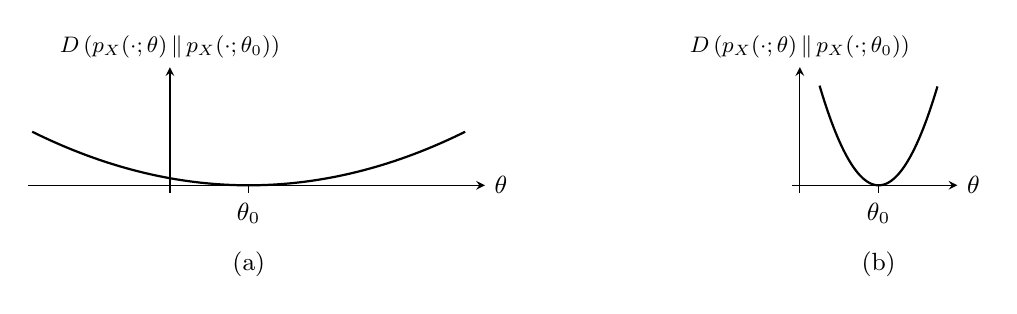
\begin{tikzpicture}
\shorthandoff{>}
%
\pgfmathsetmacro{\t}{1}
\pgfmathsetmacro{\dx}{8}
%
% peque�a curvatura
\draw[>=stealth,->] (-1.8,0)--(4,0) node[right]{\small $\theta$};
\draw[>=stealth,->] (0,-.1)--(0,1.5) node[above,scale=.9]
{\small $D\left( p_X(\cdot;\theta) \, \| \, p_X(\cdot;\theta_0) \right)$};
\draw[thick,domain=-1.75:3.75,samples=200] plot (\x,{.09*abs(\x-\t)^2});
\draw (\t,0)--(\t,-.1) node[below]{\small $\theta_0$};
%
% granda curvatura
\draw[>=stealth,->] ({-.1+\dx},0)--({2+\dx},0) node[right]{\small $\theta$};
\draw[>=stealth,->] (\dx,-.1)--(\dx,1.5) node[above,scale=.9]
{\small $D\left( p_X(\cdot;\theta) \, \| \, p_X(\cdot;\theta_0) \right)$};
\draw[thick,domain=.25:1.75,samples=200] plot ({\x+\dx},{2.25*abs(\x-\t)^2});
\draw ({\t+\dx},0)--({\t+\dx},-.1) node[below]{\small $\theta_0$};
%
\draw (\t,-1) node{\small (a)};
\draw ({\t+\dx},-1) node{\small (b)};
\end{tikzpicture} \end{center}
%
\leyenda{Caso  escalar $\Theta  \subseteq \Rset$  (para la  representaci\'on) de
  $\Dkl{}$   en  funci\'on   de  $\theta$.    (a)  Caso   con  $J_{\theta_0}(X)$
  ``peque\~no'' y (b)  caso con $J_{\theta_0}(X)$ ``grande''. En  el caso (b) la
  determinaci\'on de $\theta$  usando $\Dkl{}$ va a ser  m\'as ``sencillo'' porque
  el m\'inimo es m\'as ``picado''.}
%
\label{fig:SZ:JCurvatura}
\end{figure}

\

Un otro vinculo  entre el mundo de la informaci\'on y  la estimaci\'on aparece a
trav\'es  de la  identidad de  de Bruijn~\footnote{A  pesar de  que  tom\'o este
  nombre, esta identidad  en su primera versi\'on fue publicada  por Stam. En su
  papel~\cite{Sta59}, menciona que esta identidad fue comunicada al Profesor van
  Soest por el Profesor  de Bruijn.}~\cite{Sta59, CovTho06, Joh04, Bar84, Bar86,
  PalVer06}. Esta identidad caracterisa lo  que es conocido como canal gaussiano
figura Fig~\ref{fig:SZ:deBruijnVerdu}-(a),  \ie la  salida $Y$ es  una versi\'on
ruidosa de  la entrada.  La identidad vincula  las variaciones de  entrop\'ia de
salida con respeto al nivel de ruido, y la informaci\'on de Fisher.

\begin{teorema}[Identidad de de Bruijn]
  Sea $X$ un  vector aleatorio continuo sobre un  abierto $\Rset^d$ y admitiendo
  una matriz de covarianza, y sea $Y  = X + T \Gauss$ donde $T$ es determinista,
  $d  \times d'$  con $  d \le  d'$,  de rango  m\'aximo, y  $\Gauss$ un  vector
  gaussiano centrado y de  covarianza $\Sigma_\Gauss$, independiente de $X$ (ver
  figura  Fig.~\ref{fig:SZ:deBruijnVerdu}-(a)).    Entonces,  la  entrop\'ia  de
  Shannon y la informaci\'on de Fisher de $Y$ satisfacen
  %
  \[
  \nabla_T H(Y) = J(Y) \, T \, \Sigma_\Gauss
  \]
  %
  donde  $\nabla_T \,  \cdot$ es  la  matriz de  componentes $\frac{\partial  \,
    \cdot}{\partial  T_{i,j}}$.  Si  $T  = T(\theta)$  depende  de un  parametro
  escalar~\footnote{Si  el parametro  es  multivariado, hace  falta entender  la
    desigualdad a trav\'es de deriva  parciales con respeto a los componentes de
    $\theta$.}   $\theta$,
  %
  \[
  \frac{\partial}{\partial \theta}  H(Y) = \Tr\left( J(Y) \,  T \, \Sigma_\Gauss
    \, \frac{\partial T^t}{\partial \theta} \right)
  \]
\end{teorema}
%
\begin{proof}
  La  clave de  este resultado  viene del  hecho de  que la  densidad $p$  de $T
  \Gauss$ satisface una ecuaci\'on diferencial particular.
  %  $$\nabla_T p_{T \Gauss}(x) =  \Hess_x p_{T
  %    \Gauss}(x) \, T \, \Sigma_\Gauss$$ Esta ecuaci\'on viene de
  La  distribuci\'on de  $T \Gauss$  se escribe  $p(x) =  (2 \pi)^{-\frac{d}{2}}
  \left| T \Sigma_\Gauss T^t  \right|^{-\frac12} \exp\left( - \frac12 x^t \left(
      T  \Sigma_\Gauss T^t  \right)^{-1} x  \right)$ (el  rango m\'aximo  de $T$
  asegura que $T \Sigma_\Gauss T^t$ sea invertible).  Para una matriz invertible
  $R$,  desarollando  $|R|$  con  respecto  a  su  linea  $i$,  se  obtiene  que
  $\frac{\partial  |R|}{\partial R_{i,j}}  = R_{i,j}^*$  cofactor  de $R_{i,j}$,
  dando por la regla de Cram\'er $\nabla_R |R| = |R| \, \left( R^{-1} \right)^t$
  (ver     tambi\'en~\cite[cap.~1~\&~9]{MagNeu99}),    es     decir    $\nabla_R
  |R|^{-\frac12}  =  -\frac12   |R|^{-\frac12}  \left(  R^{-1}  \right)^t$.   De
  $\frac{\partial |R|^{-\frac12}}{\partial  T_{i,j}} = \sum_{k,l} \frac{\partial
    |R|^{-\frac12}}{\partial R_{k,l}}  \frac{\partial R_{k,l}}{\partial T_{i,j}}
  =   -\frac12    |R|^{-\frac12}   \sum_{k,l}   \left(    R^{-1}   \right)_{l,k}
  \frac{\partial  R_{k,l}}{\partial  T_{i,j}}$ con  $R  =  T \Sigma_\Gauss  T^t$
  (sim\'etrica)  y calculos  basicos  se obtiene  finalmente
  %
  \[
  \nabla_T  \left|   T  \Sigma_\Gauss  T^t  \right|^{-\frac12}  =   -  \left|  T
    \Sigma_\Gauss T^t \right|^{-\frac12} \left( T \Sigma_\Gauss T^t \right)^{-1}
  T \Sigma_\Gauss
  \]
  %
  Adem\'as,  de $\left(  T \Sigma_\Gauss  T^t \right)  \left( T  \Sigma_\Gauss T^t
  \right)^{-1}   =  I$   viene  $\frac{\partial   \left(  T   \Sigma_\Gauss  T^t
    \right)^{-1}}{\partial T_{i,j}} = -  \left( T \Sigma_\Gauss T^t \right)^{-1}
  \frac{\partial \left( T \Sigma_\Gauss  T^t \right)}{\partial T_{i,j}} \left( T
    \Sigma_\Gauss  T^t  \right)^{-1}$ donde  $e_i$  es el  vector  con  1 en  su
  componente $i$ y cero si no, dando
  %
  \begin{eqnarray*}
  \frac{\partial \left( x^t \left( T \Sigma_\Gauss T^t \right)^{-1} x
  \right)}{\partial T_{i,j}} & = & - x^t \left( T \Sigma_\Gauss T^t \right)^{-1}
  \left( e_i e_j^t \Sigma_\Gauss T^t + T \Sigma_\Gauss e_j e_i^t \right) \left( T
  \Sigma_\Gauss T^t \right)^{-1} x\\[2.5mm]
  %
  & = & - 2 \, e_i^t \left( T \Sigma_\Gauss T^t \right)^{-1} x x^t \left( T
  \Sigma_\Gauss T^t \right)^{-1} T \Sigma_\Gauss e_j
  \end{eqnarray*}
  %
  usando $x^t A e_k e_l^t  B x = e_l^t B x x^t A e_k =  e_k^t A^t x x^t B^t e_l$
  (escalares  comutan y  un  escalar es  igual  a su  transpuesta)  y usando  la
  simetria de  $T \Sigma_\Gauss T^t$.   Eso significa que
  %
  \[
  \nabla_T \left( x^t \left( T \Sigma_\Gauss T^t \right)^{-1} x \right) = - 2 \,
  \left(  T \Sigma_\Gauss  T^t \right)^{-1}  x  x^t \left(  T \Sigma_\Gauss  T^t
  \right)^{-1} T \Sigma_\Gauss,
  \]
  %
  dando
  %
  \[
  \nabla_T p(x)  = \left( - \left(  T \Sigma_\Gauss T^t \right)^{-1}  + \left( T
      \Sigma_\Gauss  T^t   \right)^{-1}  x   x^t  \left(  T   \Sigma_\Gauss  T^t
    \right)^{-1} \right) T \Sigma_\Gauss \, p(x)
  \]
  %
  Tomando la Hessiana de $p$ con  respeto a $x$ se obtiene sencillamente que $p$
  satisface  la  ecuaci\'on  diferencial
  %
  \[
  \nabla_T p = \Hess_x p \, T \, \Sigma_\Gauss
  \]
  %
  Suponiende que  se puede intervertir derivadas  y integrales (ver~\cite{Bar84,
    Bar86}  donde  se  dan   condiciones  rigorosas),  $\displaystyle  p_Y(y)  =
  \int_{\Rset^d}  p_X(x)  p(y-x)  \,   dx$  satisface  tambi\'en  la  ecuaci\'on
  diferencial, y adem\'as
  %
  \begin{eqnarray*}
  \nabla_T H(Y) & = & - \int_{\Rset^d} \nabla_T \, p_Y(y) \log p_Y(y)
  \, dy - \int_{\Rset^d} \nabla_T \, p_Y(y) \, dy\\[2.5mm]
  %
  & = & - \left( \int_{\Rset^d} \Hess_y \, p_Y(y) \log p_Y(y) \, dy \right) T \,
  \Sigma_\Gauss - \nabla_T \int_{\Rset^d} p_Y(y) \, dy\\[2.5mm]
  %
  & = & - \left( \int_{\Rset^d} \left( \Hess_y \Big( p_Y(y) \log p_Y(y) \Big) -
  \Hess_y \, p_Y(y) - \frac{\nabla_y \, p_Y(y) \, \nabla_y \, p_Y(y)^t}{p_Y(y)}
  \right) \, dy \right) T \, \Sigma_\Gauss\\[2.5mm]
  %
  & = & - \left( \int_{\Rset^d} \Hess_y \Big( p_Y(y) \log p_Y(y) \Big) \, dy -
  \int_{\Rset^d} \Hess_y p_Y(y) \, dy \right) T \, \Sigma_\Gauss \: + \: J(Y) \, T
  \, \Sigma_\Gauss
  \end{eqnarray*}
  %
  usando la  ecuaci\'on diferencial en la  secunda linea, el hecho  de que $p_Y$
  suma  a  1  en  la  tercera  linea  (su gradiente  es  cero  entonces),  y  la
  definici\'on de la matriz de Fisher en la \'ultima linea. Usando el teorema de
  la  divergencia (intergraci\'on  por  partes) aplicada  respectivamente a  los
  componentes de $\nabla_y p_Y \log  p_Y$ y $\nabla_y p_Y$, suponiendo que estos
  gradientes  se cancelan  en el  borde del  dominio de  integraci\'on,  los dos
  terminos  integrales valen cero,  lo que  cierra la  prueba de  la desigualdad
  general.   Adem\'as,  si  $T  =  T(\theta)$, la  secunda  desigualdad  sigue  de
  $\frac{\partial   \cdot}{\partial    \theta}   =   \sum_{i,j}   \frac{\partial
    \cdot}{\partial   T_{i,j}}   \frac{\partial   T_{i,j}}{\partial  \theta}   =
  \Tr\left( \nabla_T \, \frac{\partial T^t}{\partial \theta} \right)$.
\end{proof}

La  versi\'on  inicial  de la  identidad  de  de  Bruijn, con  $\Sigma_\Gauss  =
I$,
%
\[
\frac{d}{d\theta}     H(X+\sqrt{\theta}    \Gauss)    =     \frac12    \Tr\left(
  J(X+\sqrt{\theta} \Gauss) \right)
\]
%
se  recupera en el  caso particular  $T =  \sqrt{\theta} I$.   En este  caso, la
ecuac\'ion diferencial satisfada por la  densidad de probabilidad $p$ es la {\it
  ecuaci\'on  del  calor}.   Esta  desigualdad  cuantifica  las  variaciones  de
entrop\'ias   bajo   varaciones   de   ``niveles''   del  ruido   del   canal   de
comunicaci\'on. De una  forma, caracteriza la robustez del  canal con respeto al
nivel de ruido gaussiano (la gaussiana juega de nuevo un rol central ac\'a).

\

Existe una  otra forma  muy similar  de esta desigualdad  debido a  Guo, Shamai,
Verd\'u, Palomar~\cite{GuoSha05,  PalVer06}. Esta versi\'on  vincula a\'un m\'as
los  mundo  de la  informaci\'on  y  el de  la  estimaci\'on.   Del  lado de  la
comunicaci\'on, consiste a caracterisar  la informaci\'on mutua entre la entrada
$X$ de un canal  ruidoso y su salida, $Y = S X +  \Gauss$ donde $S$ coresponde a
un       pre-tratamiento       antes       de      la       salida,       figura
Fig.~\ref{fig:SZ:deBruijnVerdu}-(b).   Del lado  de la  estimaci\'on,  uno puede
querer estimar $X$  observando solamente $Y$.  Es conocido  que el estimador que
minimiza el  error cuandratico promedio  $\Esp\left[ \left\| \widehat{X}(Y)  - X
  \right\|^2   \right]$   es   la   esperanza  condicional   $\widehat{X}(Y)   =
\Esp[X|Y]$. Una caracteristica  de un estimador siendo su  matriz de covarianza,
se  notar\'a $\E(X|Y)  = \Esp\left[  \left(  X -  \Esp[X|Y] \right)  \left( X  -
    \Esp[X|Y]   \right)^2  \right]$   esta  matriz.    Sorpredentemente,  existe
tambi\'en una identidad entre \ $I(X;Y)$ \ y \ $\E(X|Y)$:
%
\begin{teorema}[Identidad de Guo--Shamai--Verd\'u]
  Sea  $X$  un  vector  aleatorio  continuo  sobre  un  abierto  $\Rset^{d'}$  y
  admitiendo una  matriz de covarianza, y  sea $Y = S  X + \Gauss$  donde $S$ es
  determinista, $d  \times d'$, y $\Gauss$  un vector gaussiano  centrado y de
  covarianza      $\Sigma_\Gauss$,      independiente      de      $X$      (ver
  figura Fig.~\ref{fig:SZ:deBruijnVerdu}-(b)). Entonces, la informaci\'on mutua entre
  \ $X$ \  e \ $Y$ y la  matriz de covarianza del estimador  de error cuadratico
  m\'inimo satisfacen
  %
  \[
  \nabla_S I(X;Y) = \Sigma_\Gauss^{-1} S \, \E(X|Y)
  \]
  %
  Si     $S    =     S(\\sigma)$    depende     de    un     parametro    escalar
  $\sigma$,
  %
  \[
  \frac{\partial}{\partial \sigma} I(X;Y) = \Tr\left( \Sigma_\Gauss^{-1} \, S \,
    \E(X|Y) \, \frac{\partial S^t}{\partial \sigma} \right)
  \]
\end{teorema}
%
\begin{proof}
  Notando  que  $p_{Y|X} (y,x)  =  (2  \pi)^{-\frac{d}{2}} \left|  \Sigma_\Gauss
  \right|^{-\frac12}  \exp\left( -\frac12  (y-S  x)^t \Sigma_\Gauss^{-1}  (y-Sx)
  \right)$ viene $\nabla_S p_{Y|X}(x,y)  = p_{Y|X}(x,y) \, \Sigma_\Gauss^{-1} (y
  - S x) x^t$  (ver unos pasos de la prueba de la  identidad de de Bruijn) as\'i
  que $\nabla_y  p_{Y|X}(y,x) = p_{Y|X}(y,x)  \, \Sigma_\Gauss^{-1} (y -  S x)$,
  dando
  %
  \[
  \nabla_S  p_{Y|X}(y,x)  = \nabla_y  p_{Y|X}(y,x)  x^t  \qquad \mbox{y}  \qquad
  \nabla_S p_{X,Y}(x,y) = \nabla_y p_{X,Y}(x,y) x^t
  \]
  %
  (multiplicando ambos lados por $p_X$. Ahora,  $I(X;Y) = H(Y) - H(Y|X) = H(Y) -
  H(\Gauss)$ (de la independencia, cuando $X =  x$, $Y = S x + \Gauss$ gaussiana
  de misma convarianza que $\Gauss$ y de promedio $S x$), as\'i que
  %
  \begin{eqnarray*}
  \nabla_S I(X;Y) & = & \nabla_S H(Y)\\[2.5mm]
  %
  & = & - \int_{\Rset^d \times \Rset^{d'}} \nabla_S \Big( p_{X,Y}(x,y) \, \log
  p_Y(y) \Big) \, dx \, dy\\[2.5mm]
  %
  & = & - \int_{\Rset^d \times \Rset^{d'}} \nabla_S \, p_{X,Y}(x,y) \, \log p_Y(y) \,
  dx \, dy - \int_{\Rset \times \Rset} p_{X|Y}(x,y) \, \nabla_S \, p_Y(y) \, dx \,
  dy\\[2.5mm]
  %
  & = & \int_{\Rset^d \times \Rset^{d'}} \nabla_y p_{X,Y}(x,y) \, x^t \log p_Y(y)
  \, dx \, dy - \int_{\Rset^d} \nabla_S p_Y(y) \, dy\\[2.5mm]
  %
  & = & - \int_{\Rset^d \times \Rset^{d'}} \nabla_y p_Y(y) x^t p_{X|Y}(x,y) \, dx
  \, dy\\[2.5mm]
  %
  & = & - \int_{\Rset^d} \nabla_y p_Y(y) \, \Esp\left[X^t | Y = y \right] \, dy
  \end{eqnarray*}
  %
  La secunda linea  viene de la escritura de $H(Y)$  usando $p_Y$ como marginale
  de $p_{X,Y}$  en $x$ y  intercambiando gradiente e  integral (ver pasos  de la
  prueba de la desigualdad de de Bruijn); la tercera de $p_{X,Y}/p_Y = p_{X|Y}$;
  en la cuarta  se usa la ecuaci\'on diferencial satisfecha  por $p_{X,Y}$ en la
  primera integral y  integrando en $x$ en la secunda  integral; la quinta linea
  se obtiene usando el teorema  de la divergencia (intergraci\'on por partes) en
  la integraci\'on en  $y$ de la primera integral,  e intercambiando gradiente e
  integral el la secunda ($p_Y$ sumando a 1, el termino se cancela). Adem\'as,
  %
  \begin{eqnarray*}
  \nabla_y p_Y(y) & = & \int_{\Rset^{d'}} \nabla_Y p_{Y|X}(y,x) \, p_X(x) \,
  dx\\[2.5mm]
  %
  & = & - \Sigma_\Gauss^{-1} \int_{\Rset^{d'}} (y - S x) \, p_{Y|X}(y,x) \, p_X(x) \,
  dx\\[2.5mm]
  %
  & = & - \Sigma_\Gauss^{-1} \left( y - S \int_{\Rset^{d'}} x \, p_{X|Y}(x,y) \,dx
  \right) p_Y(y)\\[2.5mm]
  %
  & = & - \Sigma_\Gauss^{-1} \Big( y - S \Esp\left[X | Y=y \right] \Big) \, p_Y(y)
  \end{eqnarray*}
  %
  escribiendo $p_{Y|X}(y,x)  \, p_X(x) =  p_{X|Y}(x,y) \, p_Y(y)$ en  la tercera
  linea. Esta ecuaci\'on permite escribir
  %
  \begin{eqnarray*}
  \nabla_S I(X;Y) & = & \Sigma_\Gauss^{-1} \int_{\Rset^d} \Big( y - S \Esp\left[X |
  Y=y \right] \Big) \Esp\left[X^t | Y=y \right] \, p_Y(y) \, dy\\[2.5mm]
  %
  & = & \Sigma_\Gauss^{-1} \left( \Esp\left[ Y \Esp\left[ X^t|Y \right] \right] - S
  \Esp\left[ \Esp\left[X | Y \right] \Esp\left[X | Y \right]^t \right]
  \right)\\[2.5mm]
  %
  & = & \Sigma_\Gauss^{-1} \left( \Esp\left[ Y X^t \right] - S \Esp\left[ \Esp\left[X
  | Y \right] \Esp\left[X | Y \right]^t \right] \right)\\[2.5mm]
  %
  & = & \Sigma_\Gauss^{-1} S \left( \Esp\left[ X X^t \right] - \Esp\left[
  \Esp\left[X | Y \right] \Esp\left[X | Y \right]^t \right] \right)
  \end{eqnarray*}
  %
  la \'ultima linea viniendo de $Y = S X + \Gauss$ con $\Gauss$ independiente de
  $X$ y  de promedio 0.  La  prueba se cierra notando  que $\Esp\left[ \Esp[X|Y]
  \right] = \Esp[X]$ y por  la formula de K\"onig-Huyggens. La secunda identidad
  viene  de  $\frac{\partial \cdot}{\partial  \sigma}  =  \Tr\left( \nabla_S  \,
    \frac{\partial S^t}{\partial \sigma} \right)$ (ver prueba de la identidad de
  de Bruijn).
\end{proof}
%
\noindent La primera versi\'on de esta identidad se recupera con $S = \sqrt{s}$,
$\Sigma_\Gauss  =  I$  y $X$  de  covarianza  identidad;  $s$ es  conocido  como
relaci\'on se\~nale/ruido es este caso.

Existen versiones  a\'un m\'as completas (con  gradientes con respeto  a la matriz
$\Sigma_\Gauss$ por  ejemplo) que se pueden  consultar en~\cite{Joh04, PalVer06,
  PayPal09}.

\begin{figure}[h!]
%
\begin{center} 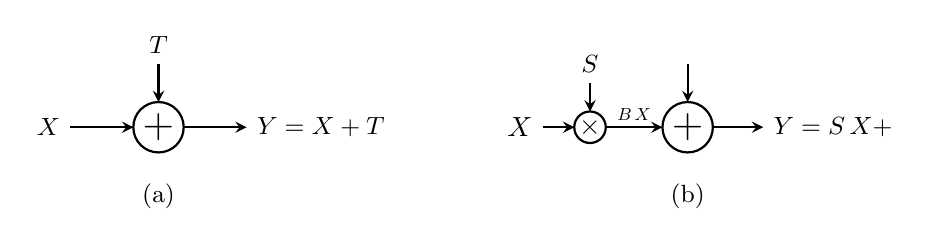
\begin{tikzpicture}[scale=.8]
\shorthandoff{>}
%
\begin{scope}
\draw[>=stealth,->,thick] (0,0) node[left]{\small $X$} --(1,0);
\draw[thick] (1.4,0) circle (.4);
\draw[>=stealth,->,thick] (1.4,1) node[above]{\small $T \N$} --(1.4,.4);
\node[align=center,scale=1.25] at (1.4,0){\large +};
\draw[>=stealth,->,thick] (1.8,0)--(2.8,0) node[right]{\small $Y = X + T \N$};
%
\end{scope}
%
\begin{scope}[xshift=7.5cm]
\draw[>=stealth,->,thick] (0,0) node[left]{$X$} --(.5,0);
\draw[thick] (.75,0) circle (.25);
\node[thick,align=center] at (.75,0){$\times$};
\draw[>=stealth,->,thick] (.75,.7) node[above]{\small $S$} --(.75,.25);
\draw[>=stealth,->,thick] (1,0)--(1.9,0);
\node[thick,align=center,scale=.7,above] at (1.45,0){\small $B \, X$};
\draw[thick] (2.3,0) circle (.4);
\draw[>=stealth,->,thick] (2.3,1) node[above]{\small $\N$} --(2.3,.4);
\node[align=center,scale=1.25] at (2.3,0){\large +};
\draw[>=stealth,->,thick] (2.7,0)--(3.5,0) node[right]{\small $Y = S \, X + \N$};
%
\end{scope}
\node at (1.4,-1.1){\small (a)};
\node at (9.8,-1.1){\small (b)};
\end{tikzpicture}
 \end{center}
%
\leyenda{Canal de comunicaci\'on gaussiano  de entrada $X$.  (a) Canal gaussiano
  usual,  donde $T$  maneja  los parametros  (nivel)  del ruido.  (b) canal  con
  gaussiano con un preprocesamiento $S$ de la entrada.}
%
\label{fig:SZ:deBruijnVerdu}
\end{figure}
\

De la desigualdad de la potencia entr\'opica  y de la identidad de de Bruijn surge
una otra desigualdad implicando la  potencia entr\'opica $N$ y la informaci\'on de
Fisher $J$. Esta desigualdad es conocida como desigualdad de Stam~\footnote{Como
  por  la identidad  de  de Bruijn,  stam  mencion\'o que  esta desigualdad  fue
  comunicada al Profesor van Soest por el Profesor de Bruijn quien da una prueba
  variacional  de  la desigualdad.}~\cite{CovTho06,  Rio07,  Sta59},  o a  veces
``desigualdad isoperimetrica para la entrop\'ia''~\cite{WanMad04}.
%
\begin{teorema}[Desigualdad de Stam]
  Sea   $X$    una   variable    aleatoria   continua   sobre    $\X   \subseteq
  \Rset^d$. Entonces,
  %
  \[
  N(X) \Tr\left( J(X) \right) \, \ge \, d
  \]
  %
  con igualdad si  y solamente si $X$ es gaussiano  de covarianza proporcional a
  la identidad.
\end{teorema}
%
\begin{proof}
  De la  desigualdad de  la potencia entr\'opica  se obtiene $N(X  + \sqrt{\theta}
  \Gauss)  \ge N(X)  + \theta  \left| \Sigma_\Gauss  \right|^{\frac1d}$. Tomando
  $\Sigma_\Gauss  = I$,  se obtiene  $\forall  \, \theta  > 0,$  \ $\frac{N(X  +
    \sqrt{\theta} \Gauss)  - N(X)}{\theta} \ge  $.  Entonces, tomando  el l\'imite
  $\theta  \to 0$,  aparece que  $\left. \frac{d}{d\theta}  N(X  + \sqrt{\theta}
    \Gauss)   \right|_{\theta  =   0}  \ge   1$.   La   prueba  se   cierra  con
  $\frac{d}{d\theta}  N(X   +  \sqrt{\theta}   \Gauss)  =  \frac{1}{2   \pi  \e}
  \frac{d}{d\theta}  \exp\left( \frac2d  H(X +  \sqrt{\theta} \Gauss)  \right) =
  \frac2d  N(X +  \sqrt{\theta}  \Gauss) \frac{d}{d\theta}  H(X +  \sqrt{\theta}
  \Gauss) = d N(X +  \sqrt{\theta} \Gauss) \Tr\left( J(X + \sqrt{\theta} \Gauss)
  \right)$  (por la identitad  de de  Bruijn).  Adem\'as,  la igualdad  se obtiene
  cuando se obtiene  la igualdad en la desigualdad de  la potencia entr\'opica, es
  decir cuando $X$ es gaussiano de  varianza proporcional a la del ruido, que es
  la identidad en este caso.
\end{proof}
%
Se  puede  ver  de  nuevo  el  rol  central  que  juega  la  gaussiana  en  esta
desigualdad. Adem\'as,  de la desigualdad de  Stam se puede  deducir tamb\'ien las
versiones escalares de la desigualdad Cram\'er-Rao. Viene del hecho de que, dado
una matriz de covarianza, le entrop\'ia  $H(X)$ es m\'axima cuando $X$ es gaussiano.
Entonces, para cualquier $X$ de covarianza $\Sigma_X$, $N(X) \le \left| \Sigma_X
\right|^{\frac1d}$,   dando  de   la  desiguldad   de  Stam,   $\left|  \Sigma_X
\right|^{\frac1d} \Tr\left( J(X) \right) \ge d$ (y las otras versiones escalares
de la relaci\'on  determinente-traza).  Como se lo puede  esperar, se obtiene la
igualdad si y solamente $X$  es gaussiana (potencia entr\'opica alcanzando su cota
superior) y de matriz la identidad (desiguladad de Stam se saturando).

Varias otras pruebas de la desigualdad de Stam pueden venir de generalizaciones,
por ejemplo debido  a Lutwak o Bercher~\cite{Lut, Ber}.  \SZ{La secci\'on ZZZ lo
  va a rapidamente evocar.}

\

\SZ{(1) Existe un data  proc ineq con Fisher, cf Rioul 07  ou Stam 59 ou Frieden
  04; cf  aussi si $I_\theta(g(X)) \le  I_\theta(X)$ used in  Kagan-Smith 1999 ;
  (2) ver MinFisher Frieden p. 235, Berchet Vignat 2009, Ernst 2017; cf. travaux
  rederivant MQ de Frieden-Plastino-Soffer  (1999, 2002), Reginato 98, Bickel 81
}